\section{Dinâmicas ou sinais de intesidade}
\index{Música!Dinâmicas}
\index{Música!Sinais de intesidade}
\label{sec:sinaisintensidade}

Em música são chamados de dinâmicas ao uso dos níveis de 
\hyperref[sec:pos:Intensidade]{\textbf{intensidade}} com que um som é gerado;
as mudanças de intensidade são indicadas mediantes símbolos, 
ou as vezes substituídos por palavras italianas ou letras;
estas modificações da intensidade vigoram até que um novo sinal seja colocado \cite[pp. 213]{medteoria} \cite[pp. 117]{mascarenhascurso}.
Quando realizamos uma modificação da intensidade, esta é chamado de ``matiz''  \cite[pp. 213]{medteoria}.

A Tabela \ref{tab:palavras:intensidade} um conjunto de palavras e letras que podemos usar 
para indicar o matiz de cada nota musical na pauta. 
\begin{table}[h]
\centering
\begin{tabular}{|p{4cm}|c|p{7cm}|}
\hline
Palavras  & Letras & Nível \\ \hline
\hline 
Fortissisimo ou molto fortissimo  & \textbf{\textit{fff}}   & Extremadamente forte. Ex: Pessoa gritando. \\ \hline
Fortissimo    & \textbf{\textit{ff}}    & Muito forte. Ex: Pessoa pouco menos que gritando. \\  \hline
Forte         & \textbf{\textit{f}}     & Forte. Ex: Pessoa falando em voz alta. \\  \hline
Mezzo forte   & \textbf{\textit{mf}}    & Meio forte. Ex: Pessoa falando.\\  \hline
Mezzo piano   & \textbf{\textit{mp}}    & Meio suave. Ex: Pessoa falando. \\  \hline
Piano         & \textbf{\textit{p}}     & Suave. Ex: Pessoa falando em voz baja. \\  \hline
Pianissimo    & \textbf{\textit{pp}}    & Muito suave. Ex: Algo mais do que um sussurro. \\  \hline
Pianissisimo ou molto pianissimo  & \textbf{\textit{ppp}}   & Extremadamente suave. Ex: Sussurrando. \\  \hline
\end{tabular}
\caption{Palavras como sinais de intensidade.}
\label{tab:palavras:intensidade}
\end{table}

\begin{example}[Indicando matizes com letras:]
A Figura \ref{fig:matiz1-1} mostra uma melodia 
que usa em todo o primeiro compasso um matiz ``piano'',
e em todo o segundo compasso um matiz ``forte''.
\end{example}
\begin{figure}[!h]
\centering
 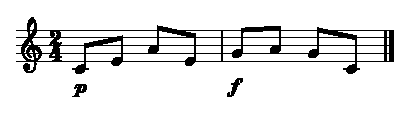
\includegraphics[width=0.7\textwidth]{chapters/cap-musica-basica/matiz1-1.eps}
\caption{Melodia com diferentes matizes.}
\label{fig:matiz1-1}
\end{figure}

Para aumentar ou diminuir gradativamente a intensidade do som,
também podem ser usados sinais ou palavras \cite[pp. 215]{medteoria} \cite[pp. 117]{mascarenhascurso}:
\begin{itemize}
\item Crescendo (cresc.); símbolo: $<$
\item Decrescendo (decresc.) ou diminuindo (dim.); símbolo: $>$
\end{itemize}

\begin{example}[Indicando matizes com letras:]
A Figura \ref{fig:matiz2-1} mostra uma melodia 
que usa em todo o primeiro compasso uma mudança gradual de matiz desde o ``piano'' até o ``forte'',
e em todo o segundo compasso uma mudança gradual do matiz desde o ``forte'' até o ``piano''.
\end{example}
\begin{figure}[!h]
\centering
 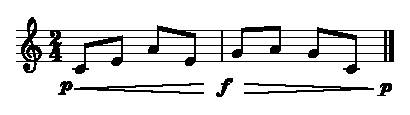
\includegraphics[width=0.7\textwidth]{chapters/cap-musica-basica/matiz2-1.eps}
\caption{Melodia com mudanças graduais de matizes.}
\label{fig:matiz2-1}
\end{figure}


%\PRLsep{Simbolos como sinais de intesidade}

